Vores marketing gør vi brug af en marketingstrategi som hedder Growth hacking, som gør brug af en del grundprincipper, som giver os muligheden at opnå et hurtigt publikum og potentielle brugere. 

Den køre på at optimere den endelige markedsføring ved brug af A/B testning, som man hurtigt kan udvikle på digitalt, som giver os muligheden for at appellere til det størst mulige publikum, derefter tager vi at optimere vores marketing baseret på Data via vores A/B teste. 

Herefter udnytter vores marketingstrategi mange forskellige kanaler såsom Sociale medier, men også E-mail marketing som at automatisere beskeder til kunder og brugere for at holde dem kroget på vores service/app. 

Denne marketsføringsstrategi har vi anset til at være den mest optimale, for vores virksomhed grundet, vores nemme tilgang til data for vores bruge, exempelvis ved brug af cookies, vi kan nemt tilpasse vores app/produkt til den individuelle brugers behov. 

Vi kan også tilpasse markedsføringen baseret på målgruppe og behov ved konstruktiv brug af data og analyse til at optimere vores marketing. 

Virksomheden kan også automatisere Data analysen og marketingsoptimeringen ved brug af Aa hvilket også er en grund til vi kommer til at anvende den for at få det mest ønskede resultat for vores virksomhed, og holder vores strategi mest optimal i forhold til fremtidig vækst 

Growth hacking kræver en specifik målsætning for vækst, vi har brug far at samle en brugerbase hurtigst muligt, så vores primære målsætning bliver at danne og skabe brugere. For at finde ud af hvordan vores bruger bliver fastholdt kan man anvende en AARRR-model til at filtrere hvor i processen vi taber flest brugere. 

AARRR-modellen opstilles således:

\textbf{Acquisition}
\begin{itemize}
    \item Folk finder vores app gennem vores digitale marketing på sociale medie platforme, som Facebook, Instagram, og Tiktok. Vi anvender deres paid marketingsystem som gør vi kan betale os til [X] antal visninger for en bestemt pris, som både giver os analytisk overblik over vores målgruppe og mængden af clicks vi får på vores reklame. Herefter kan vi analysere dataen for at opnå mere målrettet marketing.
\end{itemize}

\textbf{Activation}
\begin{itemize}
    \item Vores aktivation er hvor god en brugeroplevelse folk får så snart de trykker på vores reklame, og begynder at navigere vores app. 
\end{itemize}

\textbf{Retention}
\begin{itemize}
    \item Vores retention er primært baseret på tilbagekomst ved behov, hvis vi har en brugerflade der er nem og navigerer og giver dig brugbare resultater, vil folk automatisk vende tilbage til vores app når de har brug for at få styr på deres abonnementer igen 
\end{itemize}

\textbf{Revenue}
\begin{itemize}
    \item Vores omsætning skal meget gerne kunne betale for marketingen, samt for vedligeholdelse af vores app og server. 
    
    her kræver det, at du sætter en værdig pris for den service du udøver baseret på mængden af brugere, her tager man stilling til udbud og efterspørgelse 
    
    Hvis det her ikke fungere er det vigtigt at optimere de andre aspekter af modellen. 
\end{itemize}

\textbf{Refferal}
\begin{itemize}
    \item det vigtigste trin for alle virksomheder, hvordan dine brugere deler det med andre, hvis vores andre punkter stemmer og vi skaber en god at påpasselig brugeroplevelse eller bedre, vil folk automatisk begynde at dele det med venner og familie, man kan tjekke den data ved at se brugerene vi har fået data fra ved brug af vores markedsføring, hvis brugerne er større end mængden af tryk fra vores reklame, vores marketing været succesfuldt. 
\end{itemize}

\subsection{Konkurrentanalyse}
I takt med at abonnementsløsninger er blevet en udbredt forretningsmodel, oplever mange forbrugere, at det kan være svært at bevare overblikket over deres løbende betalinger. Dette har skabt en stigende efterspørgsel på apps, der kan hjælpe med at administrere og overvåge personlige abonnementer. 

Vi har derfor identificeret nogle af de mest relevante konkurrenter, som opererer inden for samme område som vores virksomhed. 

\vspace{2cm}
\textbf{TrackMySubs}
TrackMySubs er en amerikansk virksomhed, der tilbyder en platform, hvor brugere manuelt kan registrere deres abonnementer og modtage påmindelser inden betalinger forfalder. 

Virksomheden anvender en abonnementsbaseret prismodel, hvor funktionaliteten afhænger af, hvilken betalingsplan brugeren vælger. Dette betyder, at brugeren skal betale et ekstra abonnement for at holde styr på sine øvrige abonnementer, hvilket kan opleves som en ulempe. 

\vspace{1cm}
\textbf{Rocekt Money}
Rocket Money er ligeledes en amerikansk virksomhed, der tilbyder en app med fokus på både abonnementsoverblik og personlig økonomistyring. 

Appen giver brugeren mulighed for at: 
\begin{itemize}
\item Få overblik over aktive abonnementer  
\item Modtage notifikationer før betalinger  
\item Opsige abonnementer direkte gennem appen (via premium)  
\item Analysere forbrug, eksempelvis på dagligvarer eller cafébesøg  
\end{itemize}

Rocket Money tilbyder en premium-løsning, hvor de aktivt hjælper med at reducere brugerens udgifter, hvilket differentierer dem fra mere simple tracking-services. 

\subsubsection{Vores position i markedet}
Disse to virksomheder udgør vores primære konkurrenter, da de tilbyder lignende funktioner og henvender sig til samme målgruppe. 

Vores forretningsmodel adskiller sig dog væsentligt: 
\begin{itemize}
\item Vi anvender ikke abonnementsbetaling  
\item I stedet tilbyder vi betaling pr. analyse (engangsbetaling)  
\item Brugeren undgår dermed faste, tilbagevendende udgifter  
\end{itemize}

Dette er et centralt konkurrenceparameter, da vores løsning netop har til formål at hjælpe brugere med at reducere unødvendige abonnementer – ikke tilføje endnu et. 

Derudover planlægger vi at tilbyde: 
\begin{itemize}
\item Gratis adgang til centrale funktioner  
\item En mere fleksibel betalingsstruktur uden binding  
\end{itemize}

\subsubsection{Markedsmuligheder i Danmark}
På det danske marked findes der i øjeblikket få eller ingen stærke, lokalt forankrede løsninger med specifikt fokus på abonnementsoverblik. 

Dette giver os en potentiel \textbf{first-mover fordel}, hvor vi kan positionere os som en af de første dedikerede løsninger i Danmark. 

Det er dog vigtigt at bemærke, at internationale aktører stadig kan operere i Danmark, hvilket betyder, at vi ikke har et reelt monopol – men der er stadig gode muligheder for at opnå en stærk markedsposition gennem lokal tilpasning og målrettet markedsføring. 

\subsubsection{Kort vurdering}
Styrker ved konkurrenter:
\begin{itemize}
\item Etablerede brands  
\item Mange funktioner  
\item Dokumenteret efterspørgsel  
\end{itemize}

Vores styrker: 
\begin{itemize}
\item Ingen abonnementsbetaling  
\item Enkelt og gennemsigtigt betalingssystem  
\item Mulighed for stærk position på det danske marked 
\end{itemize}
 
\subsection{Reklamefilm}
Vi har fremstillet en reklame video, som anvender et problem $\rightarrow$ løsnings truktur, som skal highlighte problemet for vores målgruppe, hvor den herefter viser løsningen som, så er vores app.\\

Den starter med et kort segment som viser en halt masse abonnement betalinger, som der kommer flere og flere af indtil der ikke kan holdes overblik, når videoen har desorienteret seeren nok, vil den anvende en riser til en overgang, hvor der bliver snakket direkte til seeren, (vi ved godt det kan være svært), (derfor Hjælper vi) og så en overgang over til vores virksomhedsnavn og logo, og en henvisning til hvor du kan downloade den.\\

Reklame videoen har til hovedformål at vise at du potentielt kunne have et problem med abonnomenter og at du kan brænde penge af på abonnomenter.\\

Da vi målretter mod en demografi der er en lidt ældre målgruppe, har vi også fortrukket at lave videoen lidt mere simpel, som primært bare forslår en løsningsstrategi.\\

Vi har også lavet 2 forskellige videoer som en A/B test, som er blevet sendt ud igennem en spørgeundersøgelses app, hvor vi både kan få indblik i hvilken målgruppe syndes hvad, og hvilket målgrupper fortrækker hvad mest.\\

Den ene video er længere, men mere overskuelig at danne overblik over, og den anden er kortere i det første segment men går hurtigere, som skaber en større form for angst, når man ser den. 

\begin{table}[H]
    \centering
    \begin{tabular}{|l|l|l|l|l|}
        \hline
        Alder          & 15-20 år & 20 - 25 år & 25-35 år & 35+ \\ \hline
        Video A: Kort  & 43\% & 47\% & 59\% & 53\% \\ \hline
        Video B: Lang  & 57\% & 53\% & 41\% & 47\% \\ \hline
    \end{tabular}    
    \caption{Viser resultat af spørgeundnersøgelse}
\end{table}

Ud fra vores spørgeskema har vi fået en helt masse svar inden for forskellige demografer, som vi kan tage stilling ud fra. da vi prøver at målrette os målgruppen 25+, har vi valgt at starte vores kampagne med den korte video, da 59\% af dem fra 25-35 år, fortrak video A kort, da de højst sandsynligt betyder de gerne vil have pointen først, frem for et visuelt spæktakkel, men betyder også at den målgruppe genkender stressfaktoren med det samme.

Hvilket gør vores kampagne video et stærkere materiale.




\subsection{Logo og brandidentitet}
Vores logo og brandidentitet er designet til at være simpelt, moderne og let....

\subsubsection{Logo design}
Her benytter vi igen LowFi prototyping...

\begin{figure}[H]
    \centering
    \fbox{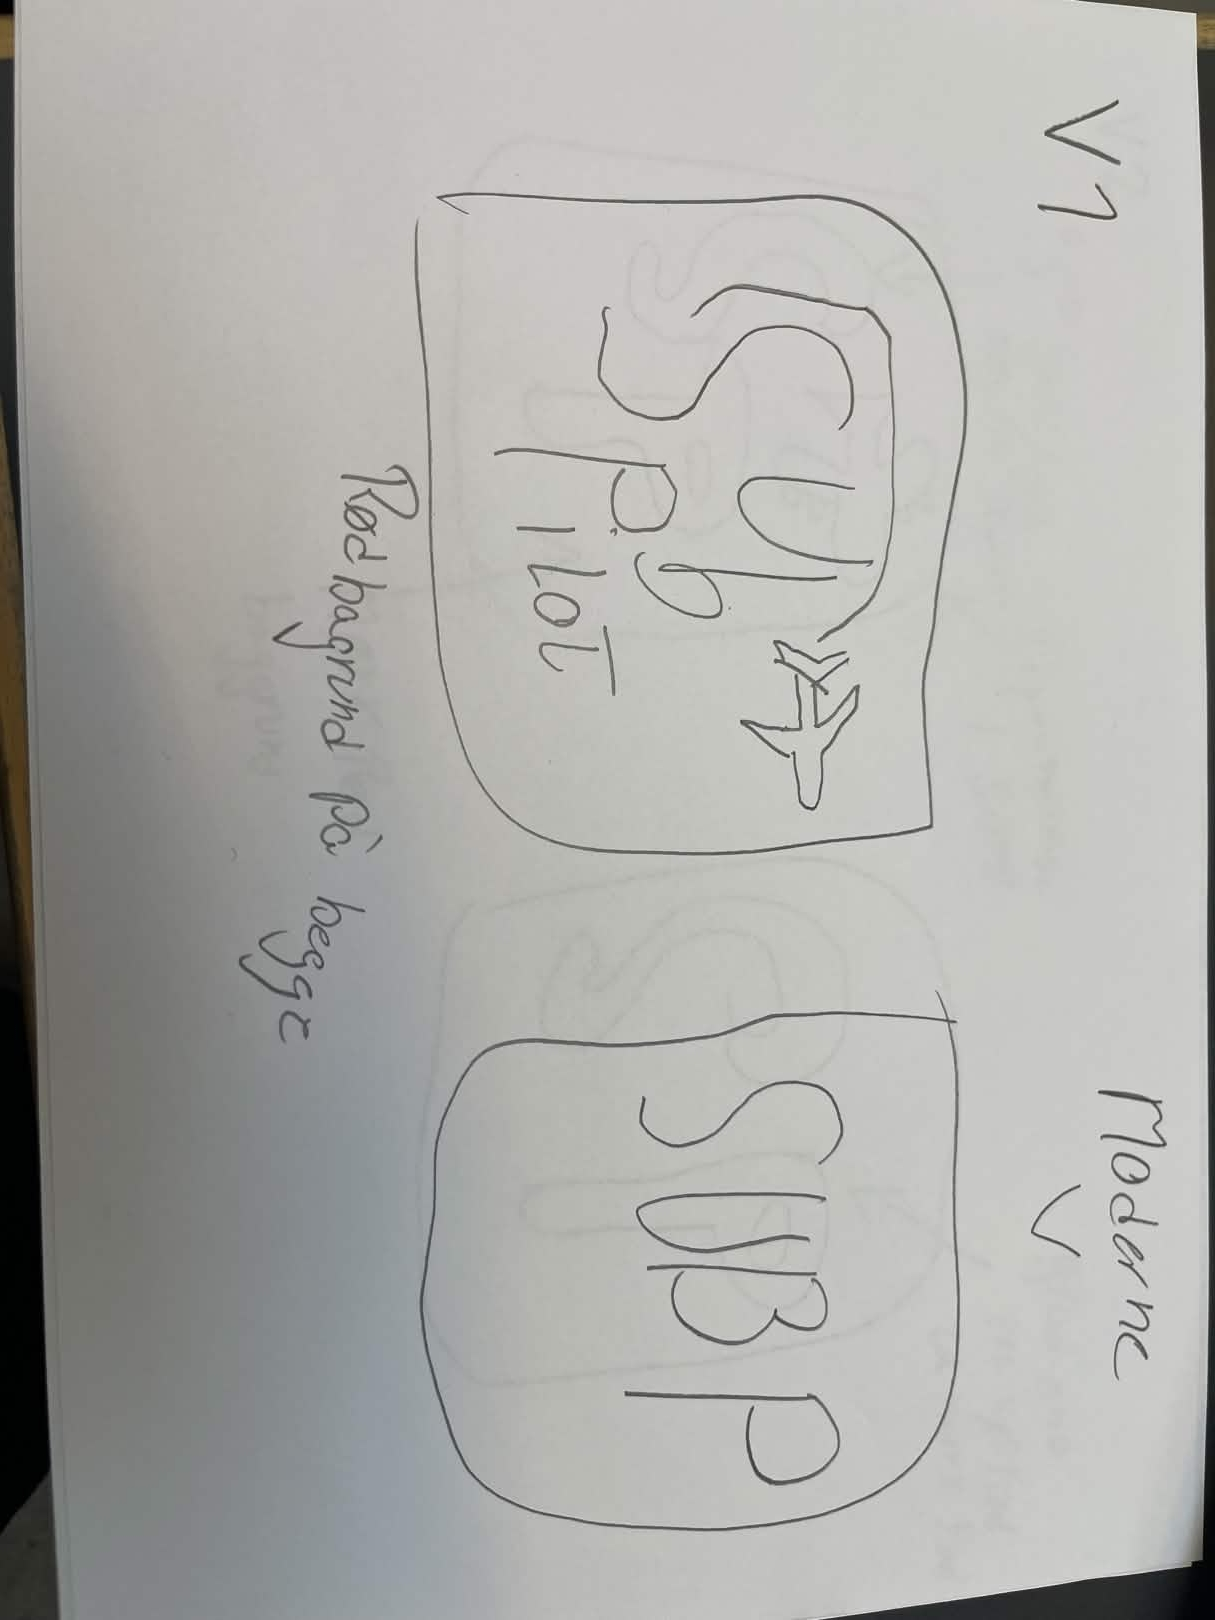
\includegraphics[width=0.7\textwidth, angle=90]{assets/skitse_v1.jpg}}
    \caption{Første iteration af LowFi prototype, lavet i hånden.}
\end{figure}

\begin{figure}[H]
    \centering
    \fbox{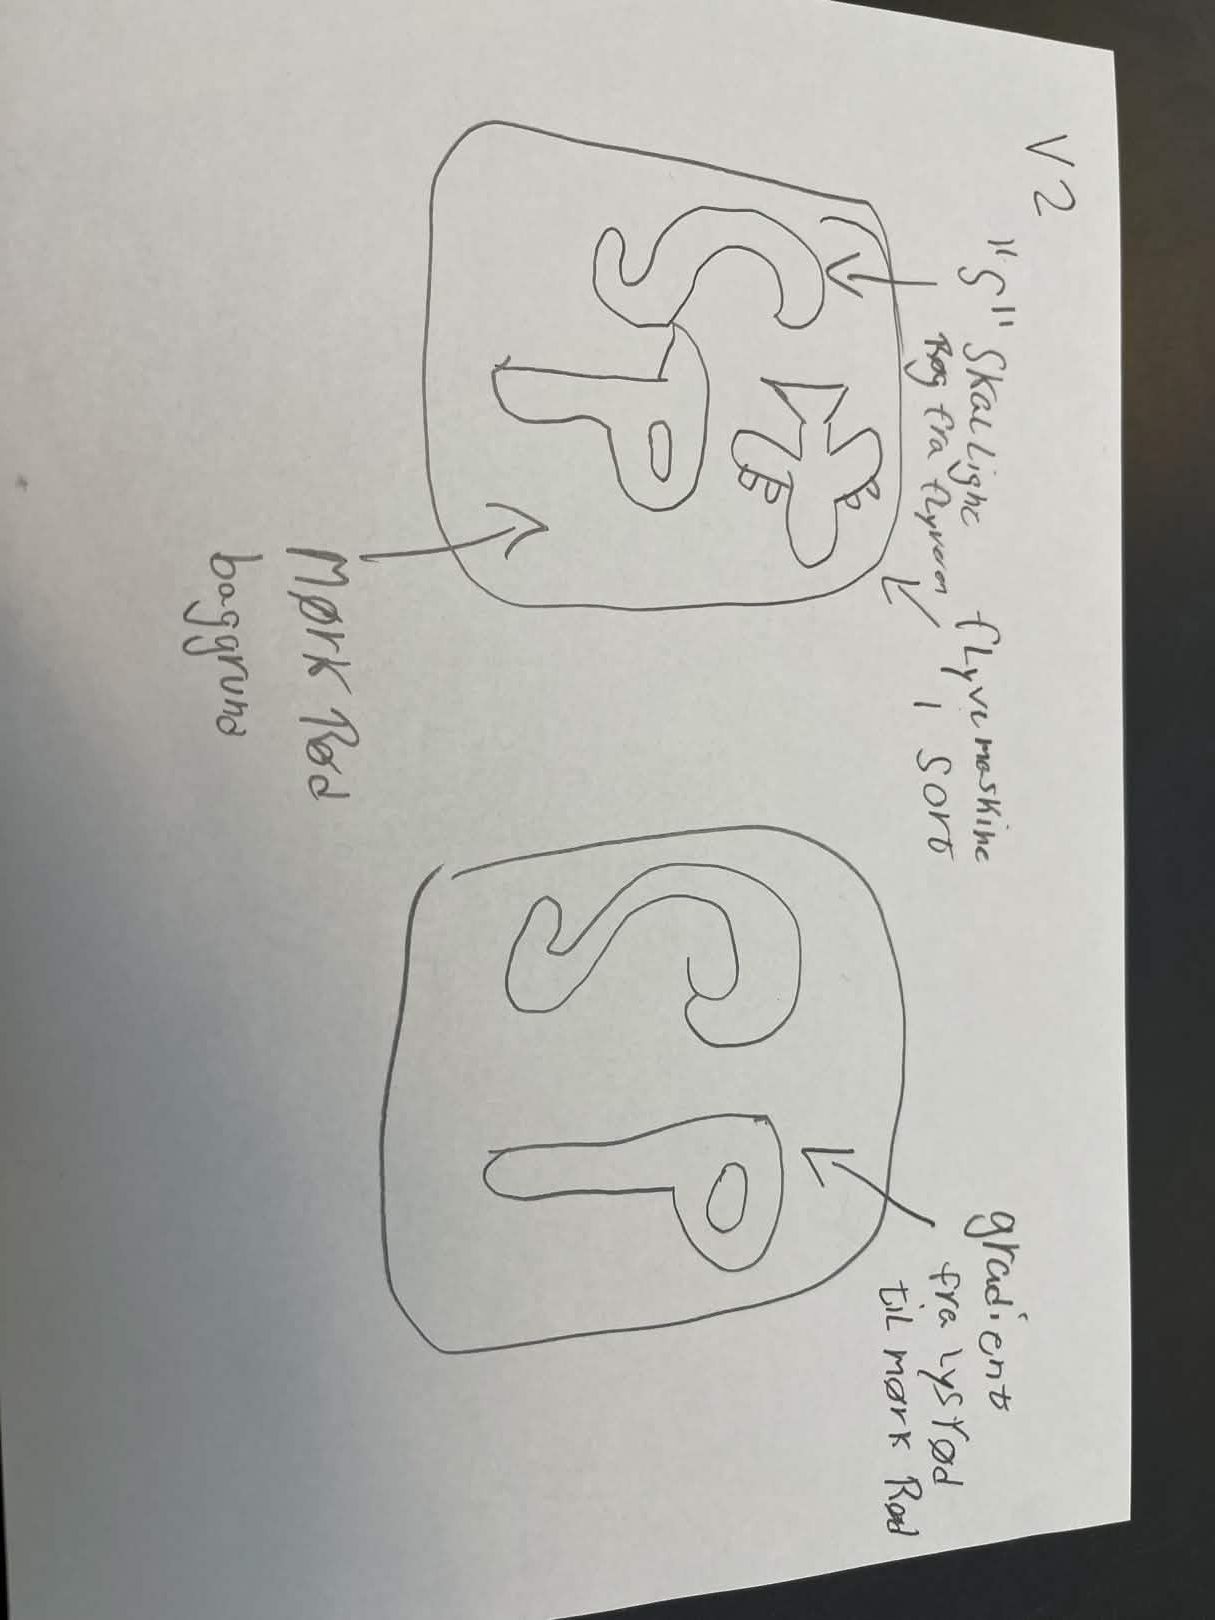
\includegraphics[width=0.7\textwidth, angle=90]{assets/skitse_v2.jpg}}
    \caption{Anden iteration af LowFi prototype, lavet i hånden.}
\end{figure}

\textbf{Endeligt logo}
\begin{figure}[H]
    \centering
    \fbox{
\includegraphics[width=0.4\textwidth]{assets/icons/red_rounded.png}}
    \caption{Endelige logo design.}
\end{figure}